\documentclass[a4paper,12pt]{report}
\usepackage[utf8]{inputenc}
\usepackage[russian]{babel}
\usepackage{graphicx}

\usepackage[left=2cm,top=2cm,right=2cm,bottom=2cm]{geometry}

\usepackage{amsmath} %для работы больших скобок в формулах и др. фич
\usepackage{amsfonts}
\usepackage{amssymb}

\usepackage{tikz} %для графиков ф-ий
\usepackage{pgfplots}
\usepackage{tkz-graph} %для графов
\usepackage{tkz-berge}

\usepackage{indentfirst} % отступ красной строки
\usepackage[unicode,colorlinks=false]{hyperref} % ссылки в оглавлении
\usepackage{mathenvrus}

\usepackage{graphicx} % для figure


\begin{document}

\author{Борис Кожуховский}
\title{Справочник по математике}
\date{2017}

\maketitle
\tableofcontents

%inlude - ставит на новую страницу
%input - просто продолжает (как будто вставляет текст из одного файла в другой)
%нельзя делать несколько вложенностей include, а input можно
\chapter*{Введение}
Цели этого справочника:\\
\begin{itemize}
	\item Систематизация и сохранение математических знаний, полученных мной за годы учёбы
	\item Сбор информации, которую трудно найти в понятном мне виде
	\item Конспектирование лекций в красивом виде
	\item Изучение LaTeX
\end{itemize} 
\chapter*{Благодарность}
Автор это справочника благодарит Максима Гунбина за предоставление некоторых материалов в уже написанном в TeX виде.

\part{Алгебра}   
\chapter{Рациональные выражения}
\section{Формулы сокращённого умножения}
\begin{itemize}
	\item $(a \pm b)^n$ вычисляется через треугольник паскаля\\
	\begin{center}
		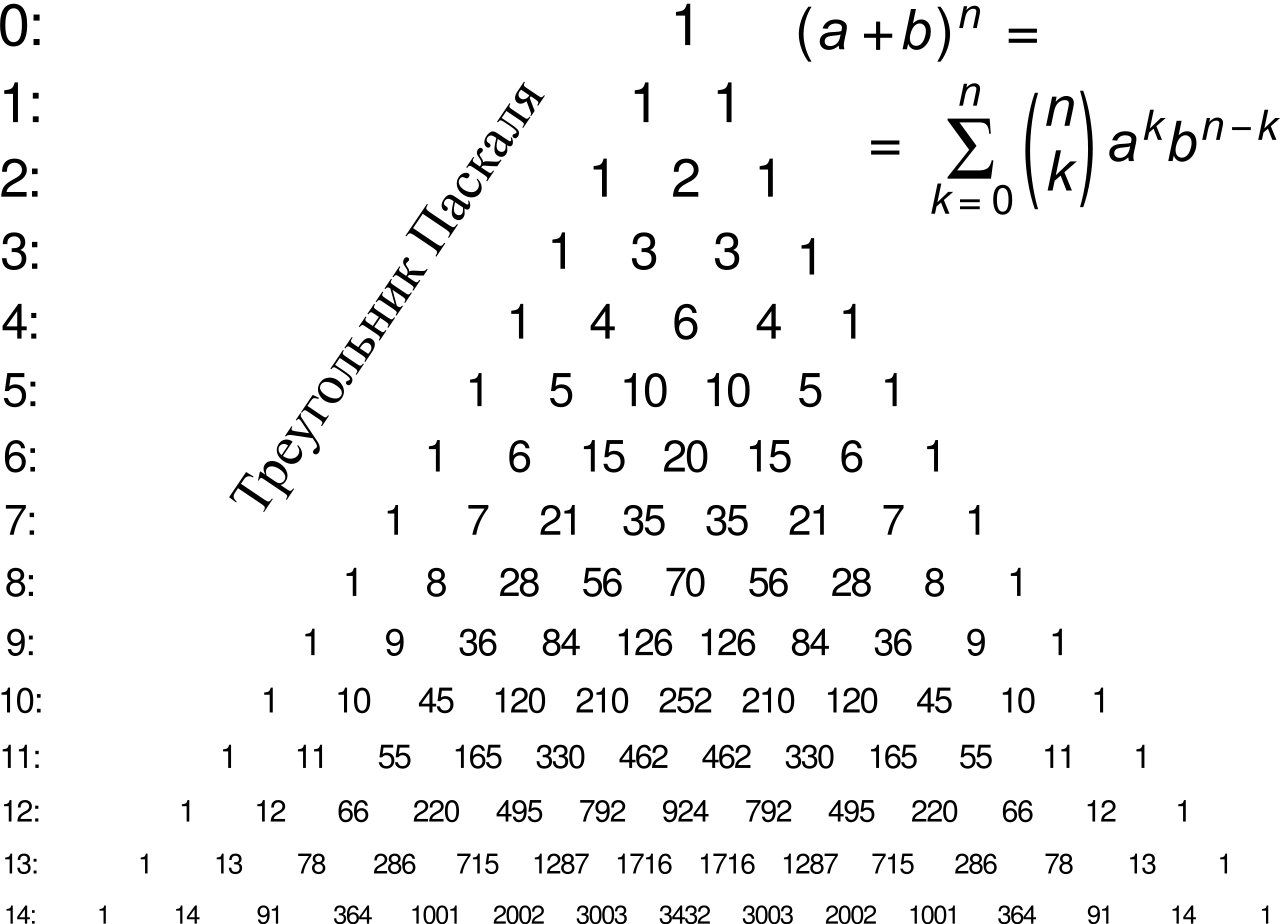
\includegraphics[scale=0.2]{./mh/algebra/rational_expressions/Pascal_triangle.png}
	\end{center}
	Например:\\
	\begin{itemize}
		\item 
	\end{itemize}
\end{itemize}           

\part{Математический анализ}
\chapter{Функции и их свойства.}
\section{График функции}
\textbf{Преобразование графиков ф-ий:}

\begin{enumerate}
	
	\item \textbf{Симметрия относительно осей координат}
	\begin{itemize}
		\item 
		Функции $y = f(x)$ и $y = -f(x)$ имеют одну и ту же область определения, их графики симметричны относительно оси $Ox$.
		%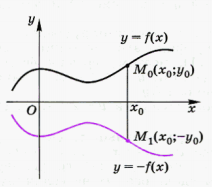
\includegraphics[scale=1]{./mh/math_analysis/functions/graph1.png}\\
		\item 
		Функции $y = f(x)$ и $y = f(-x)$ имеют области определения, симметричные относительно точки $O$. Их графики симметричны относительно оси $Oy$.
		%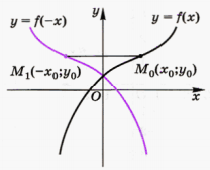
\includegraphics[scale=1]{./mh/math_analysis/functions/graph2.png}\\
	\end{itemize}

	\item \textbf{Сдвиг вдоль осей координат (параллельный перенос)}
	\begin{itemize}
		\item 
		Функция $y = f(x - a)$, где $a \neq 0$, определена для всех $x$, таких, что $(x - a) \in D(f(x))$. График ф-ии $y = f(x - a)$ 
		получается сдвигом вдоль оси $Ox$ на величину $|a|$ графика функции $y = f(x)$ вправо, если $a > 0$, 
		и влево, если $a < 0$.
		\item
		Функция $y = f(x) + B$, где $B \neq 0$, имеет ту же область определения, что и ф-ия $y = f(x)$. График ф-ии $y = f(x) + B$ 
		получается сдвигом вдоль оси $Oy$ на величину $|B|$ графика функции $y = f(x)$ вверх, если $B > 0$, 
		и вниз, если $B < 0$.
	\end{itemize}
	
	\item \textbf{Растяжение с сжатие графика вдоль всей оси координат}\\
	
	\item \textbf{Построение графика функции $y = Af(k(x - a)) + B)$ по графику функции $y = f(x)$}\\
	
	\item \textbf{Симметрия относительно прямой $y = x$}\\
	
\end{enumerate}

 %график фнкции
\section{Периодичность ф-ий}
\textbf{Определение:}\\
\textbf{\fbox{\parbox{15cm}{Функцию $y = f(x)$ с областью определения $X$ называют периодической, если 
	$\exists T \neq 0 \quad \forall x \in X$ такой, что $(x + T) \in X$, и $(x - t) \in X$, и $f(x + T) = f(x)$}}}\\

\textbf{Пример ур-ия, где используется периодичность ф-ий:}\\
Пусть $f(x)$ - периодическая функция с периодом 8, такая, что $f(x) = 8x - x^{2}$ при $x \in [0; 8)$. Решите уравнение $f(2x + 16) + 23 = 5f(x)$.\\
Решение:\\
\begin{enumerate}
	\item$$\begin{cases}
				f(x) = f(x + T) = f(x - T)\\
				T = 8\\
			\end{cases}
		 \quad \Longrightarrow \quad f(2x + 16) = f(2x)$$
	\item $x \in [0; 4) \quad \Longrightarrow \quad 2x \in [0; 8)$\\
		Решаем уравнение для этого случая:\\
		$f(2x) + 23 = 5f(x)$\\
		$16x - 4x^{2} + 23 = 40x - 5x^{2}$\\
		$x^{2} - 24x + 23 = 0$\\
		$x1 = 1$\\
		$x2 = 23\qquad \mbox{побочный корень для }x \in [0; 4)$\\
	\item $x \in [4; 8) \quad \Longrightarrow \quad (2x - 8) \in [0; 8)$\\
	Решаем уравнение для этого случая:\\
	$f(2x - 8) + 23 = 5f(x)$\\
	$16x - 64 - 4x^{2} + 16x - 64  + 23 = 40x - 5x^{2}$\\
	$x^{2} - 8x - 105 = 0$\\
	$x1 = 7$\\
	$x2 = -15\qquad \mbox{побочный корень для }x \in [4; 8)$\\
			
	\item Так как наша функция имеет период 8, то и корни будут повторятся с такой же периодичностью, так как $f(x) = f(x + T) = f(x - T)$.
	 То есть получаем корни $x = 1 + 8n$ и $x = 7 + 8n$.
\end{enumerate}
Ответ: $x = 1 + 8n$ и $x = 7 + 8n$. %периодичность
\chapter{Пределы}
\section{Предел на бесконечности}

\chapter{Производная}
\textbf{Определение:}\\
\textbf{Производной функции в точке называется предел отношения приращения функции к приращению аргумента, когда приращение аргумента стремится к 0.}\\
\textbf{\fbox{\parbox{15cm}{
			$$
			\mathbf{
			f'(x_{0}) = \lim_{\triangle x \to 0}{\frac{\triangle f}{\triangle x}} = 
			\lim_{\triangle x \to 0}{\frac{f(x_0 + \triangle x) - f(x_0)}{\triangle x}}
	     	}
			$$
			}}}\\\\
$\triangle x \qquad$ - приращение аргумента, то есть изменение аргумента от $x$ до $x_0$ (дельта $x$).\\
$\triangle f = f(x + \triangle x) - f(x) \qquad$ - приращение функции (дельта $f$).\\

\section{Свойства производных}
\textbf{
	\begin{enumerate}
		\item $ \mathbf{(C * x)' = C * (x)' \qquad C = const } $
		\item $ \mathbf{(f + g)' = f' + g' }$
		\item $ \mathbf{(f * g)' = f' * g + g' * f }$
		\item $ \mathbf{ \left(\dfrac{f}{g}\right)' = \dfrac{f' * g - g' * f}{g^2} } $
		\item $ \mathbf{ (f(g))' = f'(g) * g'(f) } $
		\item $ \mathbf{ (f^g) = f^g * \ln{f} * g' + g * f^(g - 1) * f' } \qquad $
		\item $ \mathbf{ f'(y) = \dfrac{1}{g(x)} } \qquad $
		 $\mathbf{f(y)}$ и $\mathbf{g(x)}$ - взаимообратные функции ($\mathbf{D(f(y)) = E(g(x))}$ и $\mathbf{D(g(x)) = E(f(y))}$).
	\end{enumerate}
}

\input{./mh/math_analysis/derivative/functions_extremes/2_variables}
\input{./mh/math_analysis/derivative/functions_extremes/3_variables}
\input{./mh/math_analysis/derivative/functions_extremes/conditional_extremum.tex}



\section{Геометрическая интерпретация производной}
\input{./mh/math_analysis/geometric/tangent}
\input{./mh/math_analysis/geometric/normal}

\part{Геометрия}


\part{Дискретная математика}             
\chapter{Булевы функции}

\section{Методы минимализации}
\subsection{Импликанты}
Литерал - это переменная или её отрицание. Н-р: $x_1, \overline{x_1}x_2$\\
Импликант $K$ - это такая коньюкция литералов функции $F$, что $K_i \rightarrow F_i$\\
Простой ипликант - это такой импликант, что вычеркиванием из него литералов нельзя получить новый импликант.\\
Н-р:\\
\begin{tabular}{ccccccc}
	$x_1$ & $x_2$ & $x_3$ & $K_1 = x_1$ & $K_2 = \overline{x_3}$ & $x_1x_2$ & $F$\\
	$0$ & $0$ & $0$ & $0$ & $1$ & $0$ & $0$\\
	$0$ & $0$ & $1$ & $0$ & $0$ & $0$ & $0$\\
	$0$ & $1$ & $0$ & $0$ & $1$ & $0$ & $1$\\
	$0$ & $1$ & $1$ & $0$ & $0$ & $0$ & $0$\\
	$1$ & $0$ & $0$ & $1$ & $1$ & $0$ & $1$\\
	$1$ & $0$ & $1$ & $1$ & $0$ & $0$ & $1$\\
	$1$ & $1$ & $0$ & $1$ & $1$ & $1$ & $1$\\
	$1$ & $1$ & $1$ & $1$ & $0$ & $1$ & $1$\\
\end{tabular}\\
$K_1$ - простой импликант\\
$K_2$ - не импликант\\
$K_3$ - импликант\\


\subsection{Сокращенные ДНФ}
\subsection{Тупиковые ДНФ}
\subsection{Кратчайшие и минимальные ДНФ}

\section{Классы булевых функций и полнота}
\subsection{Классы БФ}
\subsection{Теорема о функциональной полноте} 
 
\chapter{Теория графов}
\section{Основные понятия}

Два графа называются \textbf{изоморфными}, если они одинаковые с точностью до переименования вершин. % основные определения
\section{Связность графов}

Вершины $u$ и~$v$ называются \textbf{связанными}, если существует $(u, v)$-маршрут, иначе~---
\textbf{несвязанными}.



Граф называется \textbf{связным}, если в~нём любые две вершины связаны, иначе~--- \textbf{несвязным}.



Граф~$G' = (V', E')$ называется \textbf{подграфом} графа~$G = (V, E)$, если $V' \subseteq V$ и
~$E' \subseteq E$.



\textbf{Компонентой связности} графа называется его максимальный (относительно включения)
связный подграф.


\subsection{Эйлеровы графы}

Цикл, содержащий все рёбра графа, называется \textbf{эйлеровым}.



Граф, содержащий эйлеров цикл, называется \textbf{эйлеровым}.


\begin{theorem}
Связный граф эйлеров ровно тогда, когда степени всех вершин чётны.
\end{theorem}
\begin{proof}
\begin{enumerate}
	\item Пусть в~графе есть эйлеров цикл. Выберем вершину~$v_0$ в~этом цикле и~начнём обходить
	его. При~каждом посещении вершины~$v \neq v_0$ степень вершины увеличивается на~2. Т.\,о., если
	посетить её $k$~раз, то $deg v = 2k$.
	
	Для~$v_0$ степень увеличивается на~1 в~начале обхода, на~1 в~конце обхода и~на~2 при
	~промежуточных посещениях. Т.\,о., её степень чётна.
	
	\item Пусть степени всех вершин чётны. Выберём цепь~$C = v_0, e_0, v_1, e_1, \ldots, e_{k-1},
	v_k$ наибольшей длины.
	
	$v_0 = v_k$
	
	Все рёбра, инцидентные~$v_k$, присутствуют в~этой цепи. Иначе, если $e = (v_k, v)$ не~
	присутствует, то цепь~$С' = v_0, e_0, \ldots, v_k, e, v$ длиннее, что противоречит выбору $C$.
	
	$v_0 \neq v_k$. При прохождении вершины~$v_i = v_k$, $k > i > 0$, степень $v_k$ увеличивается на~2. Также проходим по ребру $e_{k-1}$, тогда степень~$v_k$ нечётна. Противоречие.
	
	Пусть найдётся ребро $e = (u, v)$, не входящее в цикл и не входящее в цепь~$C$. Существует $(v_0, u)$-маршрут. Возьмём первое ребро $e' = (v_i, v')$, не входящее в $C$. Тогда цепь
	~$C' = v', e', v_i, e_i, \ldots, e_{k-1}, v_k = v_0, e_0, v_1, e_1, \ldots, v_{i-1}$ длиннее,
	чем $C$. Противоречие.
\end{enumerate}
\end{proof}

\subsection{Алгоритм нахождения эйлерова цикла}
\begin{enumerate}
\item \textbf{Алгоритм Флери (очень медленный)}.
\begin{enumerate}
	\item Выберем произвольную вершину.
	\item Пусть находимся в вершине $v$. Выберем ребро, инцидентное ей, которое должно быть мостом, только если не осталось других рёбер.
	\item Проходим по выбранному ребру и вычёркиваем его.
	\item Повторяем, пока есть рёбра.
\end{enumerate}
\item \textbf{Алгоритм объединения циклов}.
\begin{enumerate}
	\item Выберем произвольную вершину.
	\item Выбираем любое непосещённое ребро и идём по нему.
	\item Повторяем, пока не вернёмся в начальную вершину.
	\item Получим цикл~$C$. Если он не эйлеров, то $\exists u \in C, \ \exists e = (u, u') \colon u' \notin C$. Выбираем $u$ и повторяем шаг 2. Получим цикл $C'$, рёбра которого не совпадают с рёбрами $C$, объединяем их. Повторяем шаг 4.
\end{enumerate}
\end{enumerate}


Граф называется \textbf{полуэйлеровым}, если в нём есть цепь, не являющаяся циклом и содержащая все рёбра.


\begin{theorem}[критерий полуэйлерова графа]
content...
\end{theorem}

\subsection{Гамильтоновы графы}

Простой цикл, содержащий все вершины графа, называется \textbf{гамильтоновым}.



Граф называется \textbf{гамильтоновым}, если в нём есть гамильтонов цикл.


\begin{theorem}[Дирака]
Если в графе с $n$ вершинами, $n \geqslant 3$, $\forall u \ deg u \geqslant \frac{n}2$, то граф гамильтонов.
\end{theorem}
\begin{proof}
\begin{enumerate}
	\item Докажем методом от противного, что граф связный. Пусть он несвязный. Выберем компоненту
	связности $G' = (V', E')$ с наименьшим числом вершин, тогда $|V'| \leqslant \frac{n}2$.
	Возьмём $v \in V'$, тогда $deg v \leqslant |V'| - 1 < \frac{n}2$. Противоречие с условием.
	\item Выберем цепь~$C = v_0, e_0, v_1, e_1, \ldots, e_{k-1}, v_k$ максимальной длины. Тогда все вершины, соседние с $v_0$, лежат в этой цепи, иначе можно увеличить длину цепи. Аналогично для $v_0$. Среди $v_1, v_2, \ldots, v_k$ вершин, соседних с $v_0$, не менее $\frac{n}2$.
	
	Пусть $v_i$ соседняя с $v_0$. Рассмотрим $v_{i-1}$, их не менее $\frac{n}2$, расположенных среди $v_0, \ldots, v_{k-1}$. Среди них не менее $\frac{n}2$, соседних с $v_k$. Найдётся $v_{i-1}$ такая, что $v_{i-1}$ соседняя с $v_k$. $v_i$ соседняя с $v_0$.
	
	Докажем, что $v_i, e_{i+1}, \ldots, v_k, e_k, v_{i-1}, e_{i-1}, \ldots, v_0, e_k', v_i$~---
	гамильтонов цикл, методом от противного. Предположим обратное, тогда есть вершина $u$, не входящая в цикл, и существует $(v_0, u)$-маршрут, значит, существует ребро, инцидентное одной из вершин цикла, но не входящее в него. Можно получить более длинную цепь.
\end{enumerate}
\end{proof}

\begin{theorem}[Оре, 1960]
	Если в графе с $n \geqslant 3$ вершинами для любых двух несмежных вершин $u$, $v$ $deg u + deg v \geqslant n$, то граф гамильтонов.
\end{theorem}
\begin{proof}
	\begin{enumerate}
		\item Докажем методом от противного, что граф связный. Пусть он несвязный, тогда в нём найдутся хотя бы две компоненты связности $G_1(V_1, E_1)$ и $G_2(V_2, E_2)$. Пусть $u \in V_1$, $v \in V_2$. $u$ и $v$ несмежные.
		
		$deg u \leqslant |V_1| - 1 \land deg v \leqslant |V_2| - 1 \opbr\Rightarrow deg u + deg v \opbr\leqslant |V_1| + |V_2| - 2 \opbr\leqslant n - 2$
		
		\item Докажем, что граф гамильтонов. Выберем цепь наибольшей длины $W = v_0 e_0 v_1 e_1 \ldots e_{k-1} v_k$. В~ней содержатся все вершины, соседние с~$v_0$ или~с
		~$v_k$. Т.\,о., среди вершин $v_1, \ldots, v_k$ $deg v_0$ соседних с $v_0$. Аналогично для $v_k$.
		
		$deg v_0 + deg v_k \geqslant n$, тогда найдутся $v_i$ и $v_{i+1}$ такие, что $v_i$ соседняя с $v_k$, а $v_{i+1}$~--- с $v_0$. Получили гамильтонов цикл $C = v_{i+1} e_{i+1} \ldots v_k e_k v_i e_{i-1} v_{i-1} \ldots e_0 v_0 e_k' v_{i+1}$ (доказательство аналогично доказательству в теореме Дирака).
	\end{enumerate}
\end{proof}



\textbf{Эйлеров путь} — это путь, проходящий по всем рёбрам графа и притом только по одному разу. \\
\textbf{Эйлеров цикл} — эйлеров путь, являющийся циклом. То есть замкнутый путь, проходящий через каждое ребро графа ровно по одному разу.\\
\textbf{Эйлеров граф} — граф, содержащий эйлеров цикл.\\
\textbf{Полуэйлеров граф} — граф, содержащий эйлеров путь.\\
\begin{center}
\textbf{Существование эйлерова цикла и эйлерова пути}
\end{center}
\begin{itemize}
\item В неориентированном графе\\
Согласно теореме, доказанной Эйлером, эйлеров цикл существует тогда и только тогда, когда граф связный и в нём отсутствуют вершины нечётной степени.

Эйлеров путь в графе существует тогда и только тогда, когда граф связный и содержит не более двух вершин нечётной степени.[1][2] Ввиду леммы о рукопожатиях, число вершин с нечётной степенью должно быть четным. А значит эйлеров путь существует только тогда, когда это число равно нулю или двум. Причём когда оно равно нулю, эйлеров путь вырождается в эйлеров цикл.
\end{itemize}


\textbf{Гамильтоновым циклом} является такой цикл, который проходит через каждую вершину данного графа ровно по одному разу.\\
\textbf{Гамильтонов граф} - граф, содержащий гамильтонов цикл.\\
\begin{center}
\textbf{Условия существования гамильтонова цикла в графе}
\end{center}
\begin{itemize}
\item \textbf{Условие Дирака}\\
Пусть $p$ — число вершин в данном графе и $p>3$. Если степень каждой вершины не меньше, чем $\frac{p}{2}$, то данный граф — гамильтонов. 

\item \textbf{Условие Оре}\\	
Пусть $p$ — количество вершин в данном графе и $p>2$. Если для любой пары несмежных вершин $(x, y)$ выполнено неравенство $\deg x + \deg y\geqslant p$, то данный граф — гамильтонов (другими словами: сумма степеней любых двух несмежных вершин не меньше общего числа вершин в графе).
\end{itemize}
 % связанность графов
\section{Деревья}

Граф без~циклов называется \textbf{лесом}.

Связный лес называется \textbf{деревом}.

Ребро называется \textbf{мостом}, если при~его удалении увеличивается число компонент связности.

Дерево с $n$ вершинами, которым сопоставлены числа $1, \ldots, n$, называется \textbf{помеченным}.

\begin{statement}
Ребро~--- мост ровно тогда, когда оно не~содержится в~цикле.A
\end{statement}
\begin{proof}
\begin{enumerate}
	\item Докажем методом от противного, что если ребро содержится в цикле, то оно не является мостом. Пусть ребро $e$ содержится в цикле $W = v_0 e_0 \ldots u e v \ldots v_k$, $u'$ и $v'$~--- смежные вершины.
	\begin{enumerate}
		\item Если в этом маршруте нет ребра $e$, то при его удалении из графа $u'$ и $v'$ останутся смежными.
		\item Если $u' = v_0' e_0' \ldots u e v \ldots e_m v_m' = v'$~--- маршрут, соединяющий $u'$ и $v'$, тогда при удалении $e$ из графа $u'$ и $v'$ соединяет маршрут $u' = v_0' e_0' \ldots u \ldots e_0 v_0 = v_k e_{k-1} \ldots v \ldots e_m v_m' = v'$.
	\end{enumerate}
	\item Пусть $e = (u, v)$ не является мостом, тогда $u$, $v$ лежат в одной компоненте связности. Удалим $e$ из графа, тогда число компонент связности не изменилось, значит, $u$ и $v$ также лежат в одной компоненте связности, т./,е. существует цепь, соединяющая $u$ и $v$: $u = v_0 e_0 \ldots e_{k-1} v_k = v$. Тогда в исходном графе существует цикл $u = v_0 e_0 \ldots e_{k-1} v_k = v e u$.
\end{enumerate}
\end{proof}
\begin{theorem}
Следующие утверждения о графе $G$ с $n$ вершинами эквивалентны:
\begin{enumerate}
	\item $G$~--- дерево.
	\item $G$ связный и имеет $n - 1$ ребро.
	\item $G$ связный и каждое его ребро~--- мост.
	\item $G$ не содержит циклов и имеет $n - 1$ ребро.
	\item Любые две вершины графа $G$ соединены ровно одной простой цепью.
	\item $G$ не содержит циклов и добавление ребра приводит к появлению цикла.
\end{enumerate}
\end{theorem}
\begin{proof}
\begin{itemize}
	\item Докажем 1) $\Rightarrow$ 3). Связность следует из определения дерева. В силу пред. утв. каждое ребро~--- мост.
	
	\item Докажем 3) $\Rightarrow$ 2). Связность по предположению. Докажем методом математической индукции, что в графе $n - 1$ ребро.
	\indbase Для $n = 1, 2$ очевидно.
	\indstep Пусть для графов с числом вершин, меньшим $n$,  Возьмём мост $e$ и удалим его. Получим две компоненты связности $G_1 = (V_1, E_1)$, $G_2 = (V_2, E_2)$. По предположению индукции $|E_1| = |V_1| - 1$, $|E_2| = |V_2| - 1$. В исходном графе рёбер $|E_1| + |E_2| + 1 = |V_1| + |V_2| - 1 = n - 1$.
	\indend
	
	\item Докажем 2) $\Rightarrow$ 4). В $G$ $n - 1$ ребро по предположению. Докажем методом математической индукции, что $G$ не содержит циклов.
	\indbase Для $n = 1, 2$ очевидно.
	\indstep Докажем, что в графе есть вершина степени 1. $\forall u \ deg u \geqslant 1$. $\forall u \ deg u \geqslant 2 \Rightarrow 2|E| = \sum_{u \in V} deg u \geqslant 2n \Rightarrow n - 1 = |E| \geqslant n$. Значит, в графе найдётся вершина степени 1. Удалим её и инцидентное ей ребро. Полученный граф содержит $n - 1$ вершину и удовлетворяет утверждению 2). По предположению индукции он не содержит циклов, тогда и исходный граф не содержит циклов.
	\indend
	
	\item Докажем 4) $\Rightarrow$ 5). Докажем связность методом математической индукции.
	\indbase Для $n = 1, 2$ очевидно.
	\indstep Пусть в графе $k$ компонент связности: $G_1 = (V_1, E_1)$, $G_2 = (V_2, E_2)$, \ldots, $G_k = (V_k, E_k)$. Они являются деревьями.
	\indend
	
	$|E_1| = |V_1| - 1$, $|E_2| = |V_2| - 1$, \ldots, $|E_k| = |V_k| - 1$. $n - 1 = |E_1| + \ldots + |E_k| = n - k \Rightarrow k = 1$, значит, граф связный.
	
	Пусть существуют вершины $u$, $v$ такие, что их соединяют две простые цепи, тогда в графе есть цикл, что противоречит предположению. Тогда эти вершины соединены ровно одной простой цепью.
	
	\item Докажем 5) $\Rightarrow$ 6). Предположим, что в графе есть цикл $v_0 e_0 v_1 e_1 \ldots v_k = v_0$, тогда есть две простые цепи $v_0 e_0 \ldots v_{k-1}$ и $v_{k-1} e_k v_k = v_0$, соединяющие $v_0$ и $v_{k-1}$, что противоречит предположению.
	
	Докажем, что добавление ребра приводит к появлению ровно одного цикла. Рассмотрим несоседних вершины $u$ и $v$. По предположению есть цепь $u = v_0 e_0 \ldots v_k = v$, соединяющая их. Тогда $u = v_0 e_0 \ldots v_k = v e u$~--- цикл, где $e$~--- $(u, v)$-маршрут. Пусть есть 2 цикла, соединяющих $u$ и $v$. Удалим $e$, цикл останется. Получили исходный граф, в котором нет циклов. Противоречие.
	
	\item 6) $\Rightarrow$ 1). Докажем связность. Рассмотрим вершины $u$ и $v$. Если они не соединены ребром, то соединим и по предположению получим цикл $v_0 e_0 \ldots u e v \ldots e_{k-1} v_k = v_0$. Тогда $u \ldots e_0 v_0 = v_k e_{k-1} \ldots v$~--- $(u, v)$-маршрут. Противоречие.
\end{itemize}
\end{proof}

\input{./mh/discrete_mathematics/graph/trees/spanning_tree} 


\input{./mh/discrete_mathematics/graph/trees/p_code} % коды прюфера % деревья
\section{Планарные графы}
\textbf{Плоский граф} - граф, который "нарисован" на плоскости так, чтобы ребра не пересекались.\\
\textbf{Планарный граф} - граф, который изоморфный плоскому.\\
\textbf{Грань плоского графа} - часть плоскости, границей которого являются его рёбра, и не содержащая внутри себя простых циклов.\\
\begin{center}\textbf{Формула Эйлера для плоских графов.}\end{center}
Если граф плоский, то выполняется такой равенство
$$
\mathbf{n - m + f = 2}
$$
где $n$ - число вершин, $m$ - число рёбер, $f$ - число граней.\\
Для любых планарных выполняется
$$
\mathbf{m \leq 3n - 6}
$$
где $n$ - число вершин, $m$ - число рёбер.\\
\textbf{Разбиением} графа $G$ называется граф, получающийся добавлением новой вершины на какое-нибудь ребро графа $G$.\\
Два графа называются гомеоморфными если получаются разбиением из одного и того же графа. (Стягиваем вершины степени 2 в ребро (удаляем их))\\
\begin{center}Критерий планарности. \textbf{Теорема Понтрягина-Куратовского}\end{center}
\textbf{Граф планарный тогда и только тогда, когда он не содержит подграфов, гомеоморфных $K_5$, $K_{3,3}$.} % планарные графы 

\part{Теория множеств}             
\chapter{Основные понятия}
\section{Определение}
\index{Множество}\textbf{Множество} - ключевое понятие теории множест. Оно аксиоматично, то есть неопределяемо. Обозначаются множества обычно заглавными буквами латинского алфивита.\\
 $\in$ - символ принадлежности множеству.\\
\textbf{Пустое множество} — множество, не содержащее ни одного элемента.\\
\textbf{Универсальное множество (универсум)} — множество, содержащее все мыслимые объекты. В связи с парадоксом Рассела данное понятие трактуется в настоящее время как «множество, включающее все множества, участвующие в рассматриваемой задаче».
\section{Аксиоматика}

\section{Операции на множествами}
\begin{itemize}
	\item Объеденение $A \cup B = C \quad \Leftrightarrow \quad \forall c \in C : c \in A \text{ или } c \in B$
	\item Пересечение $A \cap B = C \quad \Leftrightarrow \quad \forall c \in C : c \in A \text{ и } c \in B$
	\item Разница $A \backslash B = C \quad \Leftrightarrow \quad \forall c \in C : c \in A \text{ и } c \notin B$
	\item Симметрическая разница $A \vartriangle B = C \quad \Leftrightarrow \quad \forall c \in C : c \in A \cup \text{ и } c \notin A \cap B $
	\item Дополнение к множеству $A$ (в универсальном множестве  $M$) $\overline{A} \quad \Leftrightarrow \quad \forall x \in \overline{A}, x \in M : x \notin A$
\end{itemize}

          
\chapter{Функции над множествами}
\section{Определение}
\index{Функция}\textbf{Функцией $\mathbf{f : A \rightarrow B}$} называется правило, ставящие в соответствие каждому элементу множества $A$ единственный элемент множества $B$ ($f(a) \in B$, $a \in A$).\\
Множество $A$ - \textbf{область определения $f$}.\\
Множество $B$ - \textbf{область заначения $f$}.\\
\section{Биекции, Иньекции, Сюрьекции}
\begin{itemize}
	\item $f : A \rightarrow B$ называют \textbf{иньективной}, если $\forall x, y \in A : x \neq y \Rightarrow f(x) \neq f(y)$
	\item $f : A \rightarrow B$ называют \textbf{сюрьективной}, если $\forall b \in B \exists a \in A : f(a) = b$
	\item $f : A \rightarrow B$ называют \textbf{биньюктивной}, если она является и иньективной и сюрьективной одновременно. 
\end{itemize}


\part{Комбинаторика}       
\hypertarget{pigeonhole_principle}{\section{Принцип Дирихле}}
В комбинаторике \textbf{принцип Дирихле} — утверждение, сформулированное немецким математиком Дирихле в 1834 году, устанавливающее связь между объектами («кроликами») и контейнерами («клетками») при выполнении определённых условий. 

Наиболее тривиальная формулировка принципа Дирихле звучит так:
\begin{center}
\textit{Если кролики рассажены в клетки, причём число кроликов больше числа клеток, то хотя бы в одной из клеток находится более одного кролика.}
\end{center} % Принцип Дирихле

\end{document}\right) 